\chapter{Binäre Bäume}

\section{Lösung}

\begin{itemize}
    \item Im \textbf{worst-case} liegen Einfügeoperationen in einem binären Suchbaum in der Komplexitätsklasse $O(n)$
    \item Im \textbf{average-case} liegen Einfügeoperationen in einem binären Suchbaum in der Komplexitätsklasse $O(log n)$
\end{itemize}

Im \textbf{}


\begin{figure}
    \begin{center}
        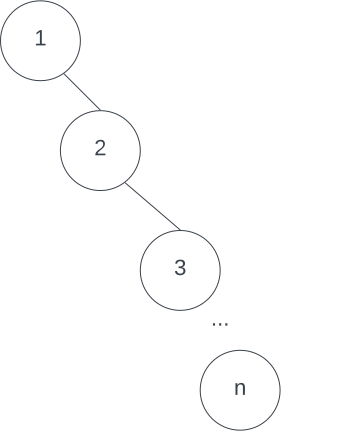
\includegraphics[scale=0.3]{chapters/5. Binäre Bäume/img/degenerate_tree}
        \caption{Für einen entarteten binären Suchbaum liegen Einfügeoperationen im \textbf{worst-case} in der Komplexitätsklasse $O(n)$ (Quelle: eigene)}
        \label{fig:degeneratetree}
    \end{center}
\end{figure}

\section{Anmerkung und Ergänzungen}


\noindent
In der Literatur wird manchmal die Definition \textbf{vollständiger} und \textbf{fast vollständiger} binärer Baum unterschiedlich gehandhabt.
Bei \textit{Ottmann und Widmayer} ist ein \textbf{vollständiger Baum} ein Baum, der auf jedem \textit{Niveau}\footnote{Knoten eines Baumes gleicher Tiefe} die maximal mögliche Knotenzahl hat und sämtliche Blätter dieselbe Tiefe haben (vgl.~\cite[261]{OW17e}).\\
Bei \textit{Güting und Dieker} entspricht die Definition der eines \textbf{fast vollständigen Baumes}, also ein Baum, der bis auf die letzte Ebene vollständig besetzt ist (vgl.~\cite[96]{GD18c}, außerdem~\cite[161]{CL22}).\\
Wir folgen der Definition von \textit{Ottmann und Widmayer} (s. Skript (Teil 2), S.  101).\\

 \noindent
Der \textbf{worst-case} ergibt sich, wenn ein binärer Suchbaum \textbf{entartet}\footnote{
\cite[136]{GD18e}
} ist - die Reihenfolge der Knoten entspricht dann der Anordnung in einer verketteten List, in der das kleinste Element am Anfang der Liste steht, das größte Element am Ende der Liste.\\
Soll jetzt ein Element eingefügt werden, dessen Schlüssel größer als alle in dem Suchbaum enthaltenen Werte ist, muss der \textit{rechte Teilbaum} bis zum Ende durchwandert werden, um das Element einzufügen.\\
Bei $n$ vorhandenen Knoten ergibt sich somit ein Zeitaufwand von $O(n)$ (Nachweis u.a. bei~\cite[135 f.]{GD18d}).\\

\noindent
Für den \textbf{average-case} stellen \textit{Sedgewick und Wayne} fest:

\blockquote[{\cite[403]{SW11}}]{
The running time of algorithms on binary search trees depend on the shapes of the trees, which, in turn, depend on the order in which keys are inserted. In the best case, a tree with $N$ nodes could be perfectly balanced [...] the balance in typical trees turns out to be much closer to the best case than the worst case.
}\\

\noindent
Ein \textbf{balancierter Baum} ist ein Baum, bei dem die Differenz der Höhe des linken Teilbaums und die Höhe des rechten Teilbaums eines Knotens max. $1$ ist (vgl. \cite[284]{OW17e}).\\
Die maximale Pfadlänge in einem balancierten Baum ist $O(log\ n)$\footnote{$n=$ Anzahl der Knoten} (vgl.\cite[135]{GD18d}).\\
Hiermit ergibt sich im \textit{ungünstigsten Fall}, dass mindestens $O(log\ n)$ Operationen nötig sind, um einen Schlüssel für eine Einfügeoperation zu finden.\\
Es läßt sich vermuten, dass mit ${k+1}$ Blättern\footnote{mit $k=$ Anzahl innere Knoten, wobei innerer Knoten $=$ Knoten mit Grad $\geq 1$} in einem vollständigen Baum im ungünstigsten Fall $(k+1) * log(n)$ Operationen nötig sind (für jedes Blatt muss einmal der komplette Pfad durchlaufen werden).\\
Eine vollständige Analyse, die für den \textbf{average-case} zu $O(log\ n)$ führt, findet sich bei \textit{Güting und Dieker} (~\cite[136 ff.]{GD18d}).























